\documentclass{res} 

\usepackage{tabularx}
\usepackage{wrapfig}
\usepackage{graphicx}

\newcommand{\frstCVcell}{2.5cm}

\setlength{\textheight}{9.5in}

\begin{document}

\moveleft.5\hoffset\centerline{\LARGE\bf Lilly Chalupowski}
\bigskip
\moveleft.5\hoffset\centerline{\large\bf Security Application Developer - Threat Intelligence}
\moveleft\hoffset\vbox{\hrule width\resumewidth height 1pt}\smallskip
\moveleft.5\hoffset\centerline{11-52 Lakefront Rd.}
\moveleft.5\hoffset\centerline{Nova Scotia, Canada, B2Y 3C6}
\moveleft.5\hoffset\centerline{+1.902.483.4267}
\moveleft\hoffset\vbox{\hrule width\resumewidth height 1pt}\smallskip

\begin{resume}

  \section{Summary}
  \line(2,0){434}
  \newline
  \newline
  In Cyber Security it's important to be versed in many different skill sets. To facilitate this skill set I've taken all Advanced Placement courses throughout High School and achieved Honors, took one year of Computer Science and four years of Engineering throughout University, have taken an additional nine courses in correspondence highlighting on White Hat Hacking,
\begin{wrapfigure}{R}{0.3\textwidth}
\centering
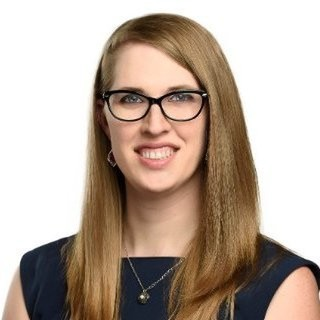
\includegraphics[width=0.28\textwidth]{../pages/index/img/profile.jpg}
Lilly Chalupowski
\end{wrapfigure}

  Web Application Security Testing, Security+ and Networking, also continuing my technical knowledge by reading books like The Shellcoders Handbook, Hacking the Art of Exploitation and Web Application Hackers Handbook.

I'm familiar with the PCI Compliance methodology and I'm able to determine if a business meets SAQ A, B, C or D. I'm able to work with ASV's to get external scans completed that meet compliance requirements as well.

I've done public relations as well delivering presentations to the consumer market as well as the private sector at the Atlantic Security Conference. These presentations include live hacking demonstrations and remediation proof of concept work. These demonstrations have included Lock Picking, SQL Injection, Buffer Overflows, Remote Exploitation, Malware, WiFi Exploitation, XSS, and more.

I also make hacking tools in my spare time one called Chameleon and one called Badger. Chameleon is a base64 Stenography Tool with Advanced Key Options and can be incorporated into AV Evasion Projects, Badger is a Windows Exploit Development Tool designed to allow easier enumeration of DEP, SEH, and ASLR protections.
\newline
\line(1,0){434}

\section{Skills}
\begin{tabularx}{\textwidth}{ X X X }
  \textbullet\ C & \textbullet\ C++ & \textbullet\ Python\\
  \textbullet\ Reverse Engineering & \textbullet\ Yara Rules & \textbullet\ Data Forensics\\
  \textbullet\ gcc & \textbullet\ Bash & \textbullet\ JavaScript\\
  \textbullet\ HTML & \textbullet\ CSS & \textbullet\ ELisp\\
  \textbullet\ Linux & \textbullet\ Gentoo & \textbullet\ PostgreSQL\\
  \textbullet\ MySQL & \textbullet\ Buffer Overflows & \textbullet\ ROP Chains\\
  \textbullet\ Heap Overflows & \textbullet\ Format Strings & \textbullet\ Apache\\
  \textbullet\ Information Security & \textbullet\ Bootstrap & \textbullet\ Networking\\
  \textbullet\ Microsoft Office & \textbullet\ Troubleshooting & \textbullet\ Public Speaking\\
  \textbullet\ PE File Structure &  \textbullet\ RIFF & \textbullet\ Subnetting\\
  \textbullet\ SQLi & \textbullet\ XSS & \textbullet\ C TCP Programming\\
  \textbullet\ Web Application Security & \textbullet\ NDA & \textbullet\ Malware Analysis\\
  \textbullet\ Threat Intelligence & \textbullet\ NIDS & \textbullet\ LIDS\\
  \textbullet\ EDR & \textbullet\ Web Design & \textbullet\ Social Engineering\\
\end{tabularx}

\pagebreak
  \section{Experience}
  \line(1,0){434}
  \newline
  \newline
  \begin{tabularx}{\textwidth}{p{\frstCVcell}Xc}
    2017 - Present & GoSecure - Security Application Developer & Dartmouth, Canada\\
    &
    \begin{itemize}
    \item Aggregation of Threat Intelligence
    \item Yara Rules
    \item Sandbox Cluster
    \item Malware Analysis
    \item Reverse Engineering
    \item Writing NIDS / LIDS Rules
    \item PostgreSQL DBM
    \item Programming Custom API
    \end{itemize}
    & \\
    2016 - 2017 & GoSecure - Cyber Security Analyst & Dartmouth, Canada\\
    &
    \begin{itemize}
    \item NIDS
    \item LIDS
    \item Managing EDR Systems
    \item Log Analysis
    \item Standard Operating Procedures
    \item SOC
    \end{itemize}
    & \\
    2014 - 2016 & Sykes - Systems Security Technician & Bridgewater, NS, Canada\\
    &
    \begin{itemize}
    \item Removal of Root-Kits, RATs and other Malware
    \item Developed SSDP Vulnerability Scanner for several CVE Database items
    \item Resolved technical issues involving network system accessibility and stability
    \item Troubleshooting client software and security issues
    \item Using CRM and Web UI databases for client data and documentation
    \item Reviewing Event Logs and other Error Logs
    \item Processed feature requests for computers, including maintained upgrades for Windows 10
    \item Administrated network systems remotely, such as computers and various network devices
    \end{itemize}
    & \\
    \end{tabularx}
    \begin{tabularx}{\textwidth}{p{\frstCVcell}Xc}
    2014 - 2014 & Freelance - File Restoration Programmer & Dartmouth, NS, Canada\\
    &
    \begin{itemize}
    \item Restored Corrupted file headers for RIFF file format
    \item Coded in C++ using file i/o
    \item Restored all original audio from what was recovered
    \item Mixed and mastered the recovered tracks
    \item Worked with client and set expectations of data recovery
    \end{itemize}
    & \\
    2012 - 2012 & HB Studios - Audio Designer & Lunenburg, NS, Canada\\
    &
    \begin{itemize}
    \item Use of internal audio development software by EA
    \item Developed internal debug GUI tool for QA Testers using Win32 API
    \item Use of internal game compilers
    \item Debugging and troubleshooting
    \item Designing and implementing game audio
    \item Sound-file database management
    \item Microsoft Office
    \item Testing game builds for quality purposes
    \end{itemize}
    & \\
    \end{tabularx}
    \begin{tabularx}{\textwidth}{p{\frstCVcell}Xc}
    2011 - 2011 & 89.3 KRock - Audio Producer & New Minas, NS, Canada\\
    &
    \begin{itemize}
    \item Operating control room
    \item Voice over post-production
    \item Sound discrimination, data entry
    \item Operated pre-amps, vocal booths, Adobe Audition, and RCS computer server
    \item Operated controls for remote talent
    \item Mixing and Mastering Advertisements for Clients
    \end{itemize}
    & \\
  \end{tabularx}
  \newline
  \line(1,0){434}

  \pagebreak
  \section{Education}
  \line(1,0){434}
  \newline
  \newline
  \begin{tabularx}{\textwidth}{p{\frstCVcell}Xc}
    2016 - Present & Udemy Academy - Continuing Security Education & Online\\
    &
    \begin{itemize}
    \item Cyber Security
    \item Cyber Security Law
    \item White Hat Hacking and Penetration Testing
    \item Mastering Python Networking and Security
    \item Certified Whit Hat Hacker Level 2
    \item Networking for Amazon's AWS Cloud
    \item Avoiding Scams
    \item Certified Web Application Security Tester
    \item Cyber Security - Devry University
    \item Private Investigator Ethics
    \item CompTIA Security+
    \end{itemize}
    & \\
    2005 - 2010 & Acadia University - Audio Engineering, Computer Science, Sociology Minor & Wolfville, NS, Canada\\
    &
    \begin{itemize}
    \item Computer Science
    \item Physics
    \item Java Programming
    \item Microsoft Office Certification
    \item Business Mathematics
    \end{itemize}
    & \\
    1998 - 2005 & Bridgewater Jr/Sr High School - Advanced Placement & Bridgewater, NS, Canada\\
    &
    \begin{itemize}
    \item AP Physics
    \item AP Mathematics
    \item AP Biology
    \item English
    \item French
    \item History
    \item Physical Education
    \item Typing Class
    \end{itemize}
    & \\
  \end{tabularx}
  \newline
  \line(1,0){434}

  \pagebreak
  \section{Volunteer}
  \line(1,0){434}
  \newline
  \newline
  \begin{tabularx}{\textwidth}{p{\frstCVcell}Xc}
    2010 - 2014 & Eastlink TV - Volunteer & Sackville, NS, Canada\\
    &
    \begin{itemize}
    \item Running XLR Cables
    \item Troubleshooting Signal Loss
    \item Operating Production Truck Mixer
    \item Heavy Lifting of Production Gear
    \end{itemize}
    & \\
    2009 - 2009 & Smile Program - Acadia University & Wolfville, NS, Canada\\
    &
    \begin{itemize}
    \item Helping Children Cope with Disabilities
    \item Managing Large Groups of Children
    \item Leading Group Activities
    \end{itemize}
    & \\
    1998 - 1998 & 4H - Volunteer & Wileville, NS, Canada\\
    &
    \begin{itemize}
    \item Highway Cleanup
    \item Fundraising for Low Income Families
    \item Public Speaking and Presentations
    \end{itemize}
    & \\
  \end{tabularx}
  \newline
  \line(1,0){434}
 
  \end{resume}
  
\end{document}